\documentclass[10pt, xcolor=dvipsnames]{beamer}
%\documentclass[10pt, xcolor=dvipsnames,notes=only]{beamer}
%\mode<presentation>
%{
\usetheme{Goettingen}
%\setbeamercovered{transparent}
%} 
\usefonttheme{professionalfonts}
%\usecolortheme{beaver}

\usepackage{setspace}
\usepackage[english]{babel}
\usepackage[latin1]{inputenc}
\usepackage{times}
\usepackage[T1]{fontenc}
\usepackage{color}
\usepackage{graphicx}
\usepackage{amssymb}
\usepackage{amsthm}
\usepackage{bm}
\usepackage{rotating}
\usepackage{ccaption}
\usepackage{booktabs}
\usepackage{lscape}
\usepackage{colortbl}
\usepackage{arydshln}
\usepackage{tabularx}
\usepackage{graphics}
\usepackage{epstopdf}

\setbeamertemplate{navigation symbols}{}
\setbeamertemplate{items}[balls]

\newenvironment{changemargin}[2]{%
  \begin{list}{}{%
    \setlength{\topsep}{0pt}%
    \setlength{\leftmargin}{#1}%
    \setlength{\rightmargin}{#2}%
    \setlength{\listparindent}{\parindent}%
    \setlength{\itemindent}{\parindent}%
    \setlength{\parsep}{\parskip}%
  }%
  \item[]}{\end{list}}

\setbeamercolor{block title}{fg=white, bg=teal}
\setbeamercolor{block body}{bg=teal!25}

\author[]{Chad Jones and Dietrich Vollrath}
\institute[Intro Growth]{Introduction to Economic Growth}
\date[]{}


\title[Schumpeter]{The Schumpeterian Model of Growth}

\begin{document}
\maketitle

\section{Setup}
\begin{frame}{Schumpeterian model of growth}
A lot like the Romer model, but with key differences in \textbf{bold}
\begin{itemize}
	\item Has all the elements of the Solow model
	\item Is specific about what $A$ means in that model
	\item $A$ \textbf{represents quality of goods, not number}
	\item Explains the dynamics of $A$ and $g_A$
	\item Explains why $g_A$ is constant along a BGP
	\item Requires effort to create the new ideas that drive $A$ and $g_A$
	\item Explains the choice involved in making that effort
	\item \textbf{Is explicit about the role of competition}
\end{itemize}
\end{frame}

\begin{frame}{The Solow part}
Much of the model starts with familiar items. Production is
\begin{equation}
	Y_t = K_t^{\alpha}\left(A_t L_{Yt}\right)^{1-\alpha}, \nonumber
\end{equation}
where $L_{Yt}$ are workers employed in producing goods and services. $L_{Rt}$ are people engaged in R\&D producing ideas, and
\begin{equation}
	L_t = L_{Yt} + L_{Rt}.
\end{equation}
denoting the ratio of R\&D workers as
\begin{equation}
	s_R = \frac{L_{Rt}}{L_t}.
\end{equation}
\end{frame}

\begin{frame}{The Solow part}
Standard parts:
\begin{itemize}
	\item Capital accumulates in the same way as in the Solow (depends on $K/AL$)
	\item Population growth is the same as in the Solow (exogenous at $g_L$)
\end{itemize}
Assuming that $g_A$ ends up constant (which we'll see) then economy ends up at steady state with a constant $K/AL$ ratio as usual.
\end{frame}

\section{Idea Accumulation}
\begin{frame}{Schumpeterian ladders}
Here the concept of innovation is in improving on an existing idea
\begin{itemize}
	\item For example, a new version of an iPhone, or a new model of a car
	\item An innovation is a step ``up'' the ladder of quality
	\item The steps are discrete, so innovation is ``lumpy''
	\item R\&D will increase the probability of taking a step
	\item This means actual growth will be lumpy (zero one year, positive the next)
	\item But the trend growth of GDP per capita will be smooth
\end{itemize}
\end{frame}

\begin{frame}{Improving an idea}
Schumpeterian mechanics for ideas are
\begin{equation}
	A_t = (1+\gamma)^{N_t}, \label{EQ_A_N}
\end{equation}
The level of productivity at time $t$ depends on 
\begin{itemize}
	\item $N_t$. The number of steps we've taken up the ladder of quality
	\item $\gamma$, the ``step size'' of each innovation. Assumed constant.
\end{itemize}
\end{frame}

\begin{frame}{Taking steps up the ladder}
The process for taking steps depends on research effort as in 
\begin{equation}
	E[dN] = \theta \frac{L_{Rt}^{\lambda}}{A_t^{1-\phi}}, \label{EQ_dotN}
\end{equation}
where
\begin{itemize}
	\item $L_{Rt}$ is the labor doing R\&D
	\item $A_t$ is the existing position on the ladder
	\item $\theta$ scales the process
	\item $\lambda$ and $\phi$ work exactly like in the Romer model
\end{itemize}
\end{frame}

\begin{frame}{Taking steps up the ladder}
A key distinction in this equation
\begin{equation}
	E[dN] = \theta \frac{L_{Rt}^{\lambda}}{A_t^{1-\phi}}, \label{EQ_dotN}
\end{equation}
is that this is the \textit{expectation} of steps, $dN$:
\begin{itemize}
	\item R\&D effort increases the probability of taking steps
	\item And the existing level, $A_t$, may make it more or less likely you jump
\end{itemize}
\end{frame}


\section{Dynamics}
\begin{frame}{The growth rate of productivity}
To get to a growth rate for produtivity, $g_A$, start with logs:
\begin{eqnarray}
	\log A_t &=& N_t \log (1+\gamma) \nonumber \\ 
	       &\approx& N_t \gamma, \nonumber
\end{eqnarray}
and take the time derivative to find
\begin{equation}
	g_A = \frac{dA}{A_t} = \gamma dN. \label{EQ_ga_dotN}
\end{equation}
The growth rate depends on the step size, and the number of steps.
\end{frame}

\begin{frame}{Expected growth}
Because the number of steps is uncertain, so is the growth rate. 
\begin{equation}
	E[g_A] = \gamma E[dN]. \label{EQ_ega_dotN}
\end{equation}
which implies that
\begin{equation}
	E[g_A] = \gamma \theta \frac{s_R^{\lambda}L_t^{\lambda}}{A_t^{1-\phi}}. \nonumber
\end{equation}
This looks a lot like the Romer model now, but with the distinction of that expectations operator. 
\end{frame}

\begin{frame}{What does growth look like?}
\begin{center}
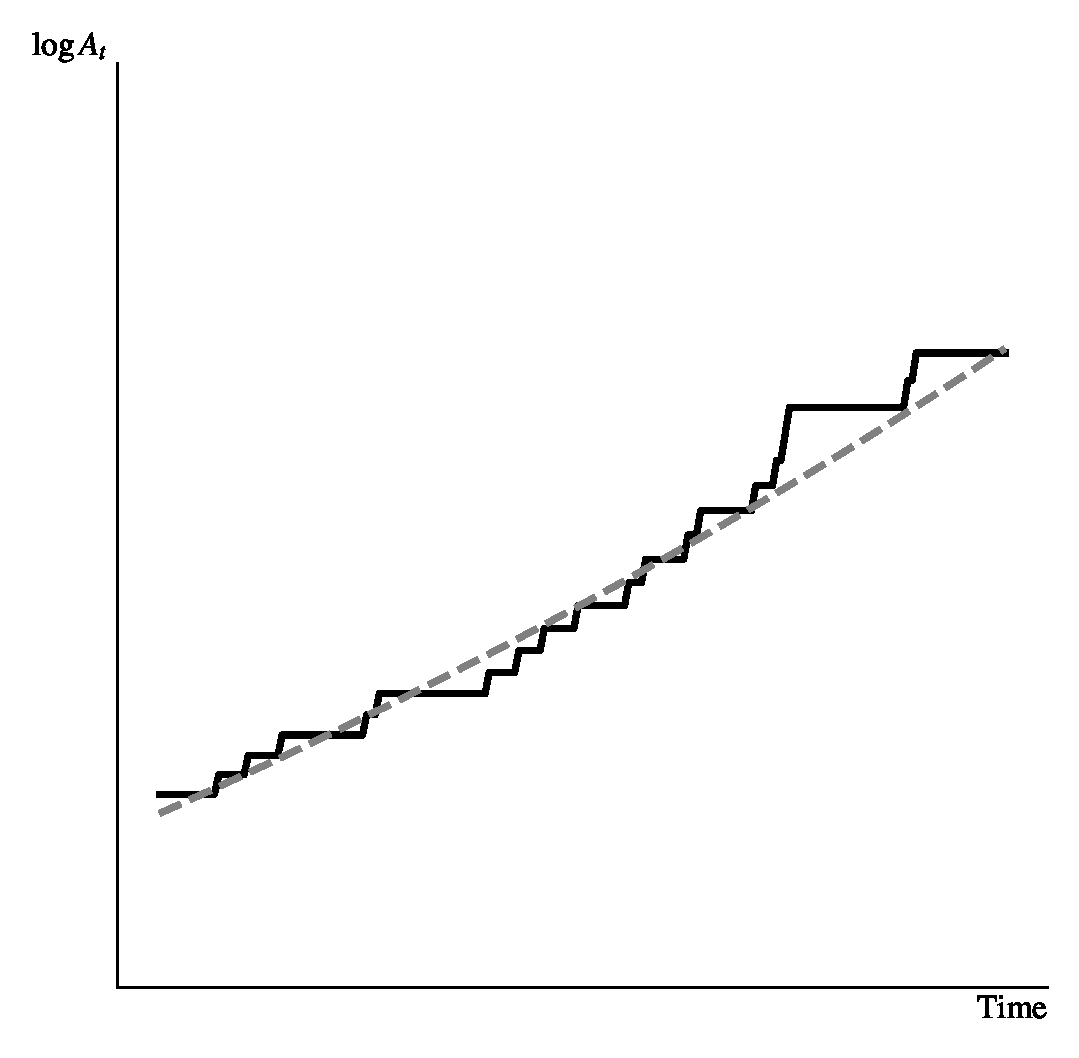
\includegraphics[height = 3in]{../Figures/fig-ch6-fig1.eps}
\end{center}
\end{frame}

\begin{frame}{Dynamics of productivity growth}
Despite the expectations operator, the long-run growth rate ends up like the Romer model
\begin{equation}
	E[g_A]^{ss} = \frac{\lambda}{1-\phi}g_L. \nonumber
\end{equation}
In expectation the growth rate still just depends on how fast the population grows. 
\end{frame}

\begin{frame}{The role of step size}
Note that in this steady state
\begin{equation}
	E[g_A]^{ss} = \frac{\lambda}{1-\phi}g_L. \nonumber
\end{equation}
The step size of innovation, $\gamma$, does not matter at all. Why?
\begin{itemize}
	\item A big $\gamma$ means big jumps in productivity, $A_t$, when innovation occurs. That should make the growth rate higher.
	\item But that same jump in $A_t$ also makes $E[dN]$ \textit{lower} because it raises the existing level of productivity
	\item These two effects cancel out in steady state. The rate at which you climb the ladder depends on how much effort you put in, $g_L$, not on how far apart the steps are, $\gamma$.
\end{itemize}
\end{frame}

\begin{frame}{The role of step size}
But note that in steady state the rate of $E[dN]$
\begin{equation}
	E[dN]^{ss} = \frac{E[g_A]^{ss}}{\gamma} = \frac{\lambda}{1-\phi}\frac{g_L}{\gamma}. \nonumber
\end{equation}
does depend on $\gamma$.
\begin{itemize}
	\item For a given level of effort, if the steps are bigger, the fewer you take. 
\end{itemize}
\end{frame}

\begin{frame}{Comparative dynamics}
All of the logic and analysis about changes in $s_R$, $\theta$, and $g_L$ are the same in the Schumpeterian model as in the Romer
\begin{itemize}
	\item There is no long-run effect on the growth rate from $s_R$. It does affect the level of $A_t$
	\item The size of $g_L$ changes the long-run growth rate and the level of $A_t$
	\item The diagram and analysis of changes is identical to the Romer model
\end{itemize}
\end{frame}

\section{R\&D Decision}
\begin{frame}{The choice of R\&D}
Like Romer, all the long-run results hold regardless of the choice of $s_R$. But $s_R$ determines the level of productivity and GDP per capita. What determines $s_R$?
\begin{itemize}
	\item How do firms make the decision to do R\&D? Fixed cost versus flow of profits
	\item What determines the fixed cost? 
	\item What determines the flow of profits?
\end{itemize}
This requires an explicit description of an imperfect market which allows market power and profits. 
\end{frame}

\begin{frame}{The cost of R\&D}
For a potential firm, the fixed cost of finding a new idea to implement is
\begin{equation}
	F_t = w_t \frac{L_{Rt}}{E[dN]}.
\end{equation}
\begin{itemize}
	\item $w_t$ is the wage they have to pay to people to do R\&D
	\item $L_{Rt}/E[dN]$ is how many workers it takes \textit{per step}
	\item Potential firms take this ratio as given, determined in the aggregate
	\item Hence $F$ is wages/worker times worker/idea = wages/idea
\end{itemize}
\end{frame}

\begin{frame}{The benefit of R\&D}
Here is where the Schumpeterian model gets interesting. 
\begin{itemize}
	\item A firm which owns the highest ``step'' on the ladder will be the one who supplies all the intermediate goods to the final goods provider. We'll show why later.
	\item A potential firm will do R\&D to try and find the next ``step'', and take over as the supplier.
	\item This is the ``creative destruction'' that Schumpeter wrote about, as one firm replaces another
	\item In Romer, all firms continued to exist forever once created - no destruction
	\item But the potential firms have to account for the chance that they will be destroyed
	\item Their eventual replacement means firms value an idea a little less, ceteris paribus
\end{itemize}

\end{frame}

\begin{frame}{The benefit of R\&D}
For a potential firm, they can earn profits from an idea but also can be replaced. They care about the present discounted value of those profits, $V$, and will compare that to $F$.
\begin{equation}
	V_0 = \pi_0 + \frac{\pi_0(1+g_{\pi})(1-E[dN])}{(1+r)} + \frac{\pi_0(1+g_{\pi})^2(1-E[dN])^2}{(1+r)^2}+ ... \nonumber
\end{equation}
\begin{itemize}
	\item $\pi_0$ is profits today
	\item $r$ is the rate of return
	\item $g_{\pi}$ is the growth rate of profits
	\item The $(1-E[dN])$ terms are the chance that the firm will be replaced in the future. Note that this probability goes up over time. Eventually they \textit{will} be replaced.
\end{itemize}

\end{frame}

\begin{frame}{The benefit of R\&D}
We can reduce that value of R\&D
\begin{equation}
	V_0 = \pi_0 + \frac{\pi_0(1+g_{\pi})(1-E[dN])}{(1+r)} + \frac{\pi_0(1+g_{\pi})^2(1-E[dN])^2}{(1+r)^2}+ ... \nonumber
\end{equation}
to 
\begin{equation}
	V_0 = \pi_0 \sum_{t=0}^{\infty} \left(\frac{1+g_{\pi}-E[dN]}{1+r}\right)^{t}, \nonumber
\end{equation}
and then
\begin{equation}
	V_0 = \frac{\pi_0}{r-g_{\pi}+E[dN]}. 
\end{equation}
\end{frame}

\begin{frame}{The innovators decisions}
We have lots of potential firms, and so long as $V_0 > F$ they will continue to do R\&D. Assume they enter until $V_0 = F$,
\begin{equation}
	\frac{\pi_t}{r-g_{\pi}+E[dN]} = w_t \frac{L_{Rt}}{E[dN]}. \nonumber
\end{equation}
Ultimately we want to solve this for $s_R$, which recall is $L_{Rt} = s_R L_t$. Like before, we are solving for $L_{Rt}$. But we need:
\begin{itemize}
	\item Initial profits
	\item Growth rate of profits
	\item Wage
\end{itemize}
\end{frame}

\section{Market Structure}
\begin{frame}{Overview}
The overall structure of this economy is both harder and easier than Romer.
\begin{itemize}
	\item At the ``top'' there are a set of final goods firms (e.g. Target). They stock \textit{one} intermediate goods that consumers purchase (e.g. just Diet Coke) 
	\item Final good firms are competitive (no profits) and there is no innovation here. They stock goods only. 
	\item There are intermediate good firms that compete to supply the single intermediate good.
	\item Each intermediate firm's product has a value of $A$ that influences the final good firm's productivity (e.g. the product is more valuable to consumers)
	\item The intermediate firm with the highest value of $A$ will supply the intermediate good
\end{itemize}
\end{frame}

\begin{frame}{Final good firms}
The final good firms produce GDP using
\begin{equation}
	Y = L_Y^{1-\alpha} A_j^{1-\alpha} x_j^{\alpha}. \label{EQ_Y_schump}
\end{equation}
\begin{itemize}
	\item $L_Y$ are production workers (not R\&D workers)
	\item $x_j$ is the amount of the product they stock
	\item $A_j$ is the \textit{level} of quality of the product they stock
	\item $\alpha$ captures how important the product is versus labor
\end{itemize}
Note that this $Y$ is GDP because intermediate good sales to the final good firm are explicitly not accounted for in GDP. 
\end{frame}

\begin{frame}{Final good maximization}
We assume final good firms maximize profits. They are competitive so profits end up at zero, but they still try. To do this they set marginal product equal marginal cost. For labor:
\begin{equation}
	w = (1-\alpha)\frac{Y}{L_Y} \label{EQ_w_schump}
\end{equation}
and for the intermediate product $j$
\begin{equation}
	p_j = \alpha L_Y^{1-\alpha} A_j^{1-\alpha} x_j^{\alpha-1}. \label{EQ_pN_schump}
\end{equation}
The important feature here is that the final good firm will pay \textit{more} for a higher quality product, $A_j$, all else equal.
\end{frame}

\begin{frame}{Intermediate good firms}
Each intermediate firm produces their good using the function $x_j = K_j$, using only capital, which costs $r$ per unit of capital. Their profits are:
\begin{equation}
	\pi_j = p_j x_j - r x_j. \nonumber
\end{equation}
\vspace{.25in}
\textbf{ASSUME} for the moment that the firm highest on the technology ladder ($N$) acts as the sole monopolist. We'll come later to why.
\vspace{.25in}
They know how $p_j$ responds to their choice of $x_j$. That is, they know what the demand curve of final good firms looks like. They set marginal revenue equal to marginal cost
\begin{equation}
	p + \frac{\partial p}{\partial x}x = r. \nonumber
\end{equation}
\end{frame}

\begin{frame}{Intermediate good firms}
Take the MR = MC condition
\begin{equation}
	p + \frac{\partial p}{\partial x}x = r. \nonumber
\end{equation}
divide by $p$
\begin{equation}
	1 + \frac{\partial p}{\partial x}\frac{x}{p} = \frac{r}{p}. \nonumber
\end{equation}
and the ratio on the left is the elasticity of price with respect to quantity, which from final goods firms is equal to $\alpha - 1$. So
\begin{equation}
	1 + (\alpha-1) = \frac{r}{p} \nonumber
\end{equation}
and we get the normal markup of
\begin{equation}
	p = \frac{1}{\alpha}r. \label{EQ_markup}
\end{equation}
\end{frame}

\section{Aggregate outcomes}
\begin{frame}{Adding up}
Given the ``micro'' results on final good firms and intermediate firms.
\begin{itemize}
	\item The best intermediate firm supplies that, $p_N = r/\alpha$
	\item Because there is one intermediate firm, it uses all capital $x_N = K$
\end{itemize}
so final good firms produce
\begin{equation}
	Y = L_Y^{1-\alpha} A_N^{1-\alpha} x_N^{\alpha}.
\end{equation}
which solves to
\begin{equation}
	Y = K^{\alpha} (A_N L_Y)^{1-\alpha}.
\end{equation}
Again this looks just like the Solow, with $A_N$ the step on the technology ladder. 
\end{frame}

\begin{frame}{Wages and profits}
Solve for things we need to know. Start with the wage. Given the first order condition from final good firms:
\begin{equation}
	w_t L_{Yt} = (1-\alpha)Y_t, \nonumber
\end{equation}
$(1-\alpha)$ of GDP gets spent on workers. The other $\alpha$ must get spent on the intermediate good (final good firms don't have profits). The revenues of the single intermediate firm are thus
\begin{equation}
	p_N x_N = \alpha Y_t
\end{equation}
\end{frame}

\begin{frame}{Profits per firm}
What are profits for the intermeidate firm?
\begin{eqnarray}
	\pi_t &=& p_t x_t - r_t x_t \nonumber \\
	      &=& (p_t - \alpha p_t) x_t \nonumber \\
	      &=& (1-\alpha) p_t x_t, \nonumber
\end{eqnarray}
and plug in for firm revenues $p_N x_N = \alpha Y_t$
\begin{equation}
	\pi_t = (1-\alpha) \alpha Y_t.\label{EQ_pi_j}
\end{equation}
are profits per intermediate firm. This is the initial profits that go into the valuation of an idea.
\end{frame}

\begin{frame}{Growth rate of profits}
How fast do profits grow? Profits are
\begin{equation}
	\pi_t = (1-\alpha) \alpha Y_t.
\end{equation}
so profits grow at the rate (along a BGP) of
\begin{equation}
	g_{\pi} = g_Y \nonumber
\end{equation}
but we know along a BGP that $g_Y = g_L + g_A$ so
\begin{equation}
	g_{\pi} = g_L + g_A
\end{equation}
or profits in the Schumpeterian model grow both with the market and as steps are taken on the ladder.
\end{frame}

\section{R\&D Solution}
\begin{frame}{Solving for $s_R$}
We have all the pieces to go back to this condition for innovation:
\begin{equation}
	\frac{\pi_t}{r-g_{\pi}+E[dN]} = w_t \frac{L_{Rt}}{E[dN]}. \nonumber
\end{equation}
so 
\begin{equation}
	\frac{\alpha(1-\alpha) Y_t}{r-g_A-g_L+E[dN]} = (1-\alpha) \frac{Y_t}{L_{Yt}} \frac{L_{Rt}}{E[dN]}. \nonumber
\end{equation}
which solves for
\begin{equation}
	\frac{s_R}{1-s_R} = \frac{\alpha(1-\alpha)}{(1-\alpha)}\frac{E[dN]}{r-g_A-g_L+E[dN]}. \nonumber
\end{equation}

\end{frame}

\begin{frame}{Solving for $s_R$}
Given
\begin{equation}
	\frac{s_R}{1-s_R} = \frac{\alpha(1-\alpha)}{(1-\alpha)}\frac{E[dN]}{r-g_A-g_L+E[dN]}. \nonumber
\end{equation}
and we know that $E[g_A] = \gamma E[dN]$ given the structure of technology, so we can arrange this to
\begin{equation}
	\frac{s_R}{1-s_R} = \frac{\alpha(1-\alpha)}{(1-\alpha)}\frac{E[dN]}{r-g_L+E[dN](1-\gamma)}. \label{EQ_sR_schump}
\end{equation}
$s_R$ is higher:
\begin{itemize}
	\item If $r$ is lower. If the future matters more, it pays to do R\&D
	\item If $g_L$ is higher. If the market will grow quickly, it pays to do R\&D
	\item If $\alpha(1-\alpha)$ (profits as a share of GDP) is higher
	\item If $(1-\alpha)$ (wages as a share of GDP) is lower
\end{itemize}
\end{frame}

\begin{frame}{Dual role of innovation}
Unlike the Romer there are two distinct effects of innovation, $E[dN]$, here:
\begin{equation}
	\frac{s_R}{1-s_R} = \frac{\alpha(1-\alpha)}{(1-\alpha)}\frac{E[dN]}{r-g_L+E[dN](1-\gamma)}. \label{EQ_sR_schump}
\end{equation}
What happens if $E[dN]$ is higher?
\begin{itemize}
	\item In the denominator, this \textit{lowers} $s_R$
	\item This captures that higher $E[dN]$ means higher chance of being replaced
	\item In the numerator, this \textit{raises} $s_R$
	\item This captures that higher $E[dN]$ makes it easier to replace the existing supplier
	\item On net, the numerator ``wins'' mathematically 
	\item Economically, the immediate gain of profits from innovation outweighs the distant chance of replacement
\end{itemize}
\end{frame}

\section{Drastic innovations}
\begin{frame}{Drastic innovation}
We assumed that the firm with the best technology was the sole monopoly provider of the intermediate good. Under what conditions does that assumption make sense?
\begin{itemize}
	\item If the ``step size'' of innovation, $\gamma$, is big enough, this will hold
	\item The final good firm values the intermediate because of the level of $A_j$ it provides
	\item The cost of producing the intermediate is the same for firms with different levels of $A_j$
	\item The final good firm will pay more for $A_N$ than for $A_{N-1}$
	\item The firm with the $A_N$ technology can lower their price until $A_{N-1}$ can't make a profit
	\item That leaves $A_N$ firm as the only supplier
	\item This only works if the step size is sufficiently large
\end{itemize}

\end{frame}

\begin{frame}{Competition}
Formally, let the $A_N$ and $A_{N-1}$ firms engage in Bertrand competition. They set prices separately, but understand the behavior of the other, and act strategically. They set their price knowing how the other firm will react. 
\vspace{.25in}\noindent Compare the demand curves for their products. For a given quantity of $x_j$, what is the relative price that the final good firm will pay for the better technology
\begin{eqnarray}
	\frac{p_N}{p_{N-1}} &=& \frac{\alpha L_Y^{1-\alpha} A_N^{1-\alpha} x^{\alpha-1}}{\alpha L_Y^{1-\alpha} A_{N-1}^{1-\alpha} x^{\alpha-1}} \nonumber \\ 
	&=& \left(\frac{A_N}{A_{N-1}}\right)^{1-\alpha} \nonumber \\ 
	&=& (1+\gamma)^{1-\alpha}. \nonumber
\end{eqnarray}
which depends on how big the step size is. 
\end{frame}


\begin{frame}{Strategic interactions}
Think through the interaction:
\begin{itemize}
	\item The lagging firm wants to stay in business. They can try to lower their price and steal the business from the leading firm. 
	\item The lagging firm lowers their price, the leading firm will follow, maintaining a ratio of $(1+\gamma)^{1-\alpha}$ so that the final good firm chooses their product
	\item The lagging firm lowers again, and the leader follows, and so on
	\item The lagging firm has to stop lowering when $p_{N-1} = r$, or when the price they charge equal MC and leaves them with zero profits
	\item We know the leading firm will charge at \textit{most} $p_N = (1+\gamma)^{1-\alpha}r$ because of the lagging firm pushing down the price
\end{itemize}
\end{frame}

\begin{frame}{Strategy for $N$}
We know $N$ firm will charge at most $p_N = (1+\gamma)^{1-\alpha}r$
\begin{itemize}
	\item If they charge exactly this then the lagging firm can still sell some units to the final good firm 
	\item if the leading firm lowers the price further, they can take all the business.
	\item Will the leading firm go lower? 
	\item The leading firm's profit-maximizing price is $p_N = r/\alpha$ as the monopolist
	\item If $r/\alpha < (1+\gamma)^{1-\alpha}r$ the profits are higher with the lower price
	\item The leading firm will set $p_N = r/\alpha$ if $(1+\gamma) > (r/\alpha)^{1/(1-\alpha)}$. 
	\item If the step size $\gamma$ is ``drastic'', then the leading firm lowers $p_N$ until the lagging firm is out of business.
	\item The assumption of a single monopolist is an assumption that innovation is ``drastic'' and that $\gamma$ is large
\end{itemize}
\end{frame}

\end{document}